\subsection{Geometria}
\label{sec:teogeom}

\begin{figure}
	\center
	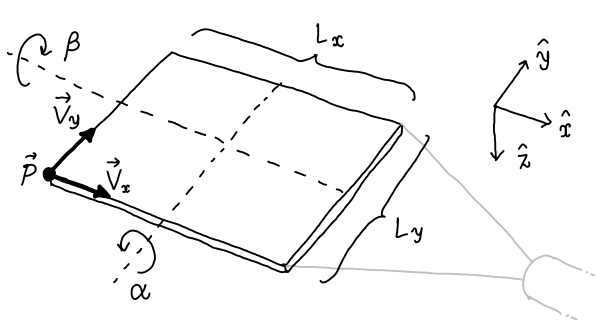
\includegraphics[width=25em]{geometriadef}
	\caption{\label{fig:geometriadef}
	Definizione del modello geometrico.
	Gli angoli $\alpha$ e $\beta$ sono nulli
	quando il lato della lastra ortogonale al loro asse di rotazione è orizzontale.
	Gli assi di rotazione sono riferiti alla lastra.}
\end{figure}

Esponiamo la modellizzazione geometrica dell'apparato ai fini di calcoli e simulazioni
(vedi \autoref{fig:geometriadef}).
Consideriamo ogni lastra di scintillatore come un parallelepipedo.
Teniamo conto dei \emph{disallineamenti} cioè della posizione arbitraria nello spazio delle lastre,
supponendo però che sia poco diversa da quella ideale di lastre orizzontali, rettangolari e allineate verticalmente.
Chiamiamo $x$ la direzione orizzontale parallela ai tubi fotomoltiplicatori,
$y$ quella ortogonale,
$z$ la direzione verticale.
Assumiamo che la direzione verticale data dalla gravità
coincida con la media dei versori normali alle lastre.

Una lastra è descritta da un'\emph{origine} $\vec P$,
da due \emph{generatori} $\hat V_x$ e $\hat V_y$
e dalle lunghezze dei lati $L_x$ e $L_y$.
La superficie superiore della lastra è un parallelogramma descritto parametricamente da
\marginpar{Mettere il simbolo di versore anche nella figura.}
\begin{equation}
	\label{eq:lastra}
	\vec r(t_x, t_y) = \vec P + t_x L_x \hat V_x + t_y L_y \hat V_y,
	\quad t_x,t_y \in (0,1).
\end{equation}

\subsubsection{Monte Carlo}

Quello che dobbiamo calcolare sono accettanze geometriche
e fattori di conversione da rate a rate per unità di area orizzontale.
Implementiamo il calcolo con un integrale Monte Carlo.

\paragraph{Raggi}

Estraiamo dei \emph{raggi} casuali.
Un raggio è definito dalle variabili aleatorie:
\begin{equation*}
	\begin{array}{ll}
		t_x, t_y & \text{uniformi in $(0,1)$}, \\
		\phi     & \text{uniforme in $(0,2\pi)$}, \\
		u        & \text{distribuzione non fissata in $(0,1)$}.
	\end{array}
\end{equation*}
Scegliamo una certa lastra che chiamiamo \emph{pivot}.
Da un raggio otteniamo una retta nello spazio parametrizzata come
\begin{align*}
	\vec r(t) &= \vec p + t \hat v, \quad \text{dove} \\
	\vec p    &= \vec r_\text{pivot}(t_x, t_y), \\
	\hat v    &= \sin\theta\cos\phi\,\hat x + \sin\theta\sin\phi\,\hat y + \cos\theta\,\hat z, \\
	\theta    &= \arccos u,
\end{align*}
e $\vec r_\text{pivot}$ è la parametrizzazione del pivot secondo la \eqref{eq:lastra}.

\paragraph{Accettanza}

Un'\emph{accettanza geometrica} è la probabilità
che un raggio che passa per il pivot
faccia scattare alcune lastre (lastre in \emph{coincidenza})
e non altre (lastre in \emph{anticoincidenza}).
Richiediamo che il pivot sia sempre in coincidenza.
Ogni lastra ha un'\emph{efficienza},
cioè la probabilità che un raggio che passa per la lastra la faccia scattare.
Sia $i$ un indice che corre lungo $N$ estrazioni di raggi casuali.
Sia $\epsilon(L)$ l'efficienza della lastra $L$.
Sia
\begin{equation*}
	w_i(L) = \begin{cases}
		1 & \text{se il raggio $i$ passa per la lastra $L$,} \\
		0 & \text{se non passa.}
	\end{cases}
\end{equation*}
Allora l'espressione che converge in probabilità all'accettanza geometrica è
\begin{align}
	\label{eq:accettanza}
	Q &:= \frac1N \sum_i q_i, \\
	\text{dove}\quad q_i &:= 
	\left( \prod_\text{$L$ in coinc.} w_i(L) \epsilon(L) \right)
	\cdot \left( \prod_\text{$L$ in anticoinc.} \big(1 - w_i(L) \epsilon(L)\big) \right). \notag
\end{align}

\paragraph{Area orizzontale}

Chiamiamo \emph{espressione logica} una specificazione di quali lastre sono in (anti)coincidenza.
Per convertire il rate di una certa espressione logica in un rate per unità di area orizzontale,
dobbiamo tener conto del fattore di conversione (il jacobiano)
dalla distribuzione con cui abbiamo estratto i raggi a una distribuzione uniforme sul piano $(x,y)$,
e della misura della parte di spazio in cui abbiamo estratto i raggi,
quindi alla fine il fattore di conversione è l'area orizzontale del pivot,
ovvero
\begin{equation*}
	A_\text{hor} = L_x \sqrt{1-(\hat V_x\hat z)^2} \cdot L_y \sqrt{1-(\hat V_y\hat z)^2},
\end{equation*}
dove i simboli hanno lo stesso significato che nella \eqref{eq:lastra}
e sono riferiti al pivot.
Detto $R$ il rate, il rate per unità di area orizzontale è dato da $R/A_\text{hor}$.

\paragraph{Incertezza}

Notiamo che la $Q$ (equazione \ref{eq:accettanza}) è una media aritmetica,
quindi una buona stima della sua varianza $\sigma_Q^2$ si ottiene con la varianza campione
\begin{equation*}
	\hat\sigma_Q^2
	= \frac1{N(N-1)} \sum_i (q_i - Q)^2.
\end{equation*}
